\documentclass[a4paper,12pt]{article}
\usepackage{amsmath,amssymb,amsfonts,amsthm}
\usepackage{tikz}
\usepackage [utf8x] {inputenc}
\usepackage [T2A] {fontenc} 
\usepackage[russian]{babel}
\usepackage{cmap, upgreek}
\usepackage{textcomp} 


% Так ссылки в PDF будут активны
\usepackage[unicode]{hyperref}

% вы сможете вставлять картинки командой \includegraphics[width=0.7\textwidth]{ИМЯ ФАЙЛА}
% получается подключать, как минимум, файлы .pdf, .jpg, .png.
\usepackage{graphicx}
% Если вы хотите явно указать поля:
\usepackage[margin=1in]{geometry}
% Или если вы хотите задать поля менее явно (чем больше DIV, тем больше места под текст):
% \usepackage[DIV=10]{typearea}

\usepackage{fancyhdr}

\newcommand{\bbR}{\mathbb R}%теперь вместо длинной команды \mathbb R (множество вещественных чисел) можно писать короткую запись \bbR. Вместо \bbR вы можете вписать любую строчку букв, которая начинается с '\'.
\newcommand{\eps}{\varepsilon}
\newcommand{\bbN}{\mathbb N}
\newcommand{\dif}{\mathrm{d}}

\newtheorem{Def}{Определение}


\pagestyle{fancy}
\makeatletter % сделать "@" "буквой", а не "спецсимволом" - можно использовать "служебные" команды, содержащие @ в названии
\fancyhead[L]{\footnotesize Электричество и магнетизм}%Это будет написано вверху страницы слева
\fancyhead[R]{\footnotesize ФМХФ МФТИ}
\fancyfoot[L]{\footnotesize \@author}%имя автора будет написано внизу страницы слева
\fancyfoot[R]{\thepage}%номер страницы —- внизу справа
\fancyfoot[C]{}%по центру внизу страницы пусто

\renewcommand{\maketitle}{%
	\noindent{\bfseries\scshape\large\@title\ \mdseries\upshape}\par
	\noindent {\large\itshape\@author}
	\vskip 2ex}
\makeatother
\def\dd#1#2{\frac{\partial#1}{\partial#2}}


\title{3.2.5 \\ Вынужденные колебания в электрическом контуре}
\author{Егор Берсенев} 
\date{15 апреля 2016 г.}

\begin{document}
	\maketitle
	\section{Цель работы}
		 Исследование вынужденных колебаний и процессов их установления
	\section{Оборудование}
		Генератор звуковой частоты, осциллограф, вольтметр, частотомер, ёмкость, индуктивность, магазин сопротивлений, универсальный мост.
	\section{Теоретическая часть}
		При подключении к колебательному контуру внешнего источника, в нем возникают колебания, которые можно представить как суперпозицию двух синусоид: первая, с частотой собственных колебаний и амплитудой, экспоненциально убывающей со временем, вторая с частотой внешнего источника и постоянной амплитудой. Со временем внешние колебаний <<забивают>> собственные, и в контуре устанавливаются только внешние колебания. Амплитуда таких колебаний максимальна при совпадении их частоты с собственной частотой контура. Зависимость амплитуды установившихся колебаний от частоты носит название резонансной кривой. Для исследования резонансной кривой будем снимать зависимость напряжения на резисторе R от частоты при постоянной амплитуде. По этим данным построим резонансную кривую. Её ширина определяет важную характеристику --- добротность. Добротность можно определить и другим способом. Например, по скорости нарастания амплитуды вынужденных колебаний. Нарастание и затухание колебаний можно наблюдать если на контур подаются цуги. Количественные оценки в таком случае можно получить, рассчитав логарифмический декремент затухания.
		
	\section{Ход работы}
		Соберем экспериментальную установку:
		
		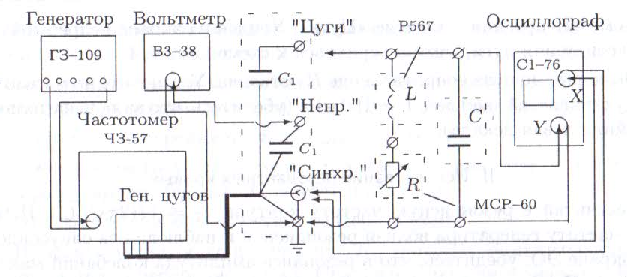
\includegraphics[width = 0.7\linewidth]{scheme1}
		
		\subsection{Исследование резонасных кривых}
		
		\begin{figure}[h!]
			\begin{minipage}[h]{0.49\linewidth}
				\centering
				R = 0 Ом

					\begin{tabular}{|l|l|l|l|}
						\hline \hline
						$f$    & $U$     & $f/f_0$ & $u/u_0$ \\ \hline
						1463 & 2,33  & 0,943  & 0,222  \\ \hline
						1479 & 2,83  & 0,953  & 0,269  \\ \hline
						1490 & 3,33  & 0,960  & 0,316  \\ \hline
						1496 & 3,67  & 0,964  & 0,348  \\ \hline
						1506 & 4,33  & 0,970  & 0,411  \\ \hline
						1505 & 4,33  & 0,970  & 0,411  \\ \hline
						1515 & 5,33  & 0,976  & 0,506  \\ \hline
						1517 & 5,67  & 0,977  & 0,538  \\ \hline
						1522 & 6,33  & 0,981  & 0,601  \\ \hline
						1533 & 8,33  & 0,988  & 0,791  \\ \hline
						1538 & 9,33  & 0,991  & 0,886  \\ \hline
						1541 & 9,67  & 0,993  & 0,918  \\ \hline
						1552 & 10,53 & 1,000  & 1,000  \\ \hline
						1562 & 9,33  & 1,006  & 0,886  \\ \hline
						1566 & 8,67  & 1,009  & 0,823  \\ \hline
						1573 & 7,33  & 1,014  & 0,696  \\ \hline
						1578 & 6,67  & 1,017  & 0,633  \\ \hline
						1586 & 5,67  & 1,022  & 0,538  \\ \hline
						1593 & 5,00  & 1,026  & 0,475  \\ \hline\hline
					\end{tabular}
						\newline \newline \newline \newline 	\newline \newline \newline \newline 
			\end{minipage}
			\hfill
			\begin{minipage}[h]{0.49\linewidth}
				
				\centering
				R = 100 Ом
				
						\begin{tabular}{|l|l|l|l|}
							\hline\hline
							$f$    & $U$     & $f/f_0$ & $u/u_0$ \\ \hline
							1597 & 2,8 & 1,03   & 0,93   \\ \hline
							1608 & 2,7 & 1,04   & 0,90   \\ \hline
							1629 & 2,5 & 1,05   & 0,83   \\ \hline
							1680 & 2,2 & 1,08   & 0,73   \\ \hline
							1685 & 2   & 1,08   & 0,67   \\ \hline
							1712 & 1,8 & 1,10   & 0,60   \\ \hline
							1746 & 1,6 & 1,12   & 0,53   \\ \hline
							1767 & 1,5 & 1,14   & 0,50   \\ \hline
							1821 & 1,3 & 1,17   & 0,43   \\ \hline
							1951 & 1   & 1,26   & 0,33   \\ \hline
							2136 & 0,8 & 1,38   & 0,27   \\ \hline
							3172 & 0,5 & 2,04   & 0,17   \\ \hline
							1553 & 3   & 1,00   & 1,00   \\ \hline
							1520 & 2,7 & 0,98   & 0,90   \\ \hline
							1502 & 2,6 & 0,97   & 0,87   \\ \hline
							1485 & 2,4 & 0,96   & 0,80   \\ \hline
							1469 & 2,2 & 0,95   & 0,73   \\ \hline
							1455 & 2   & 0,94   & 0,67   \\ \hline
							1438 & 1,8 & 0,93   & 0,60   \\ \hline
							1418 & 1,6 & 0,91   & 0,53   \\ \hline
							1408 & 1,5 & 0,91   & 0,50   \\ \hline
							1383 & 1,3 & 0,89   & 0,43   \\ \hline
							1352 & 1,1 & 0,87   & 0,37   \\ \hline
							1332 & 1   & 0,86   & 0,33   \\ \hline
							1288 & 0,8 & 0,83   & 0,27   \\ \hline
							1225 & 0,6 & 0,79   & 0,20   \\ \hline\hline
						\end{tabular}	
			\end{minipage}
			\hfill
		\end{figure}
		
		
		R = 0 Ом
		
		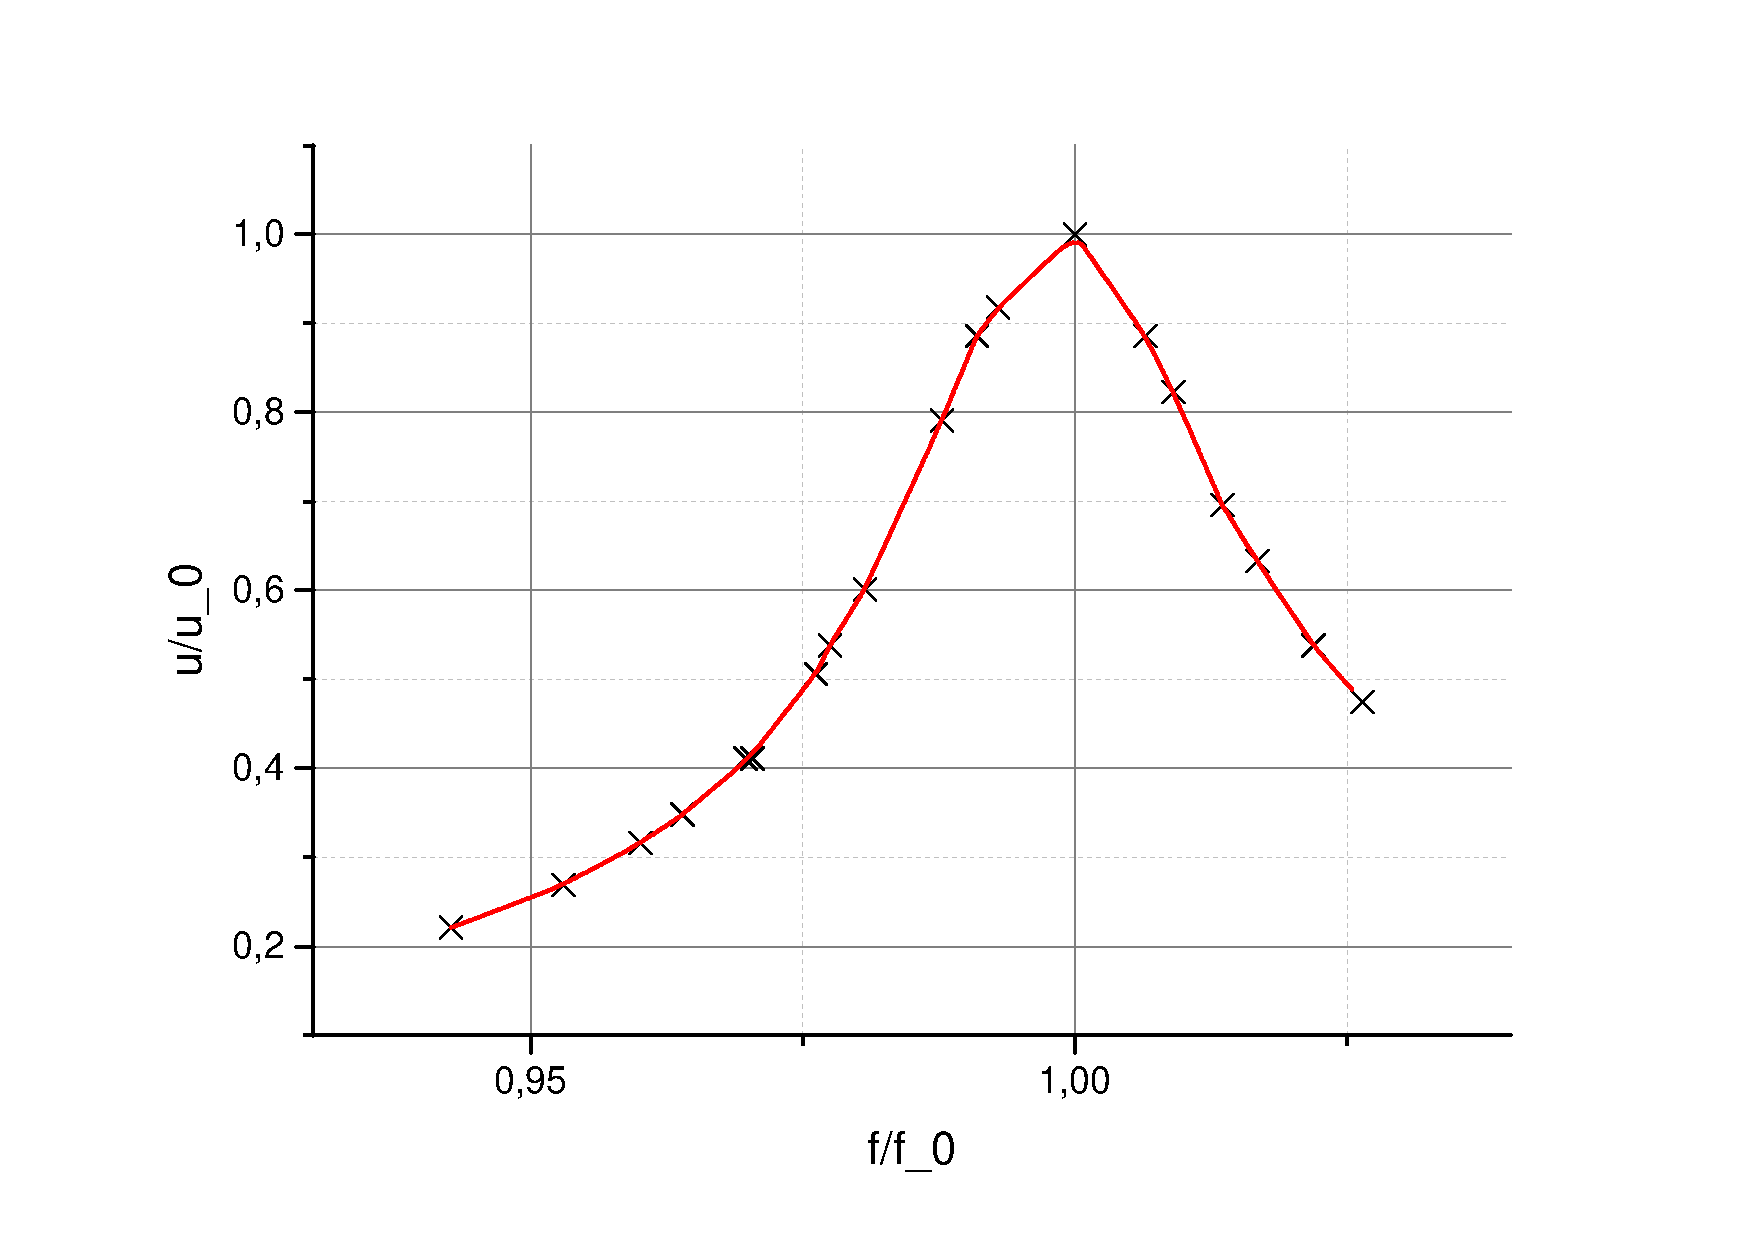
\includegraphics[width = 0.7\linewidth]{graph1}
		
		R = 100 Ом
		
		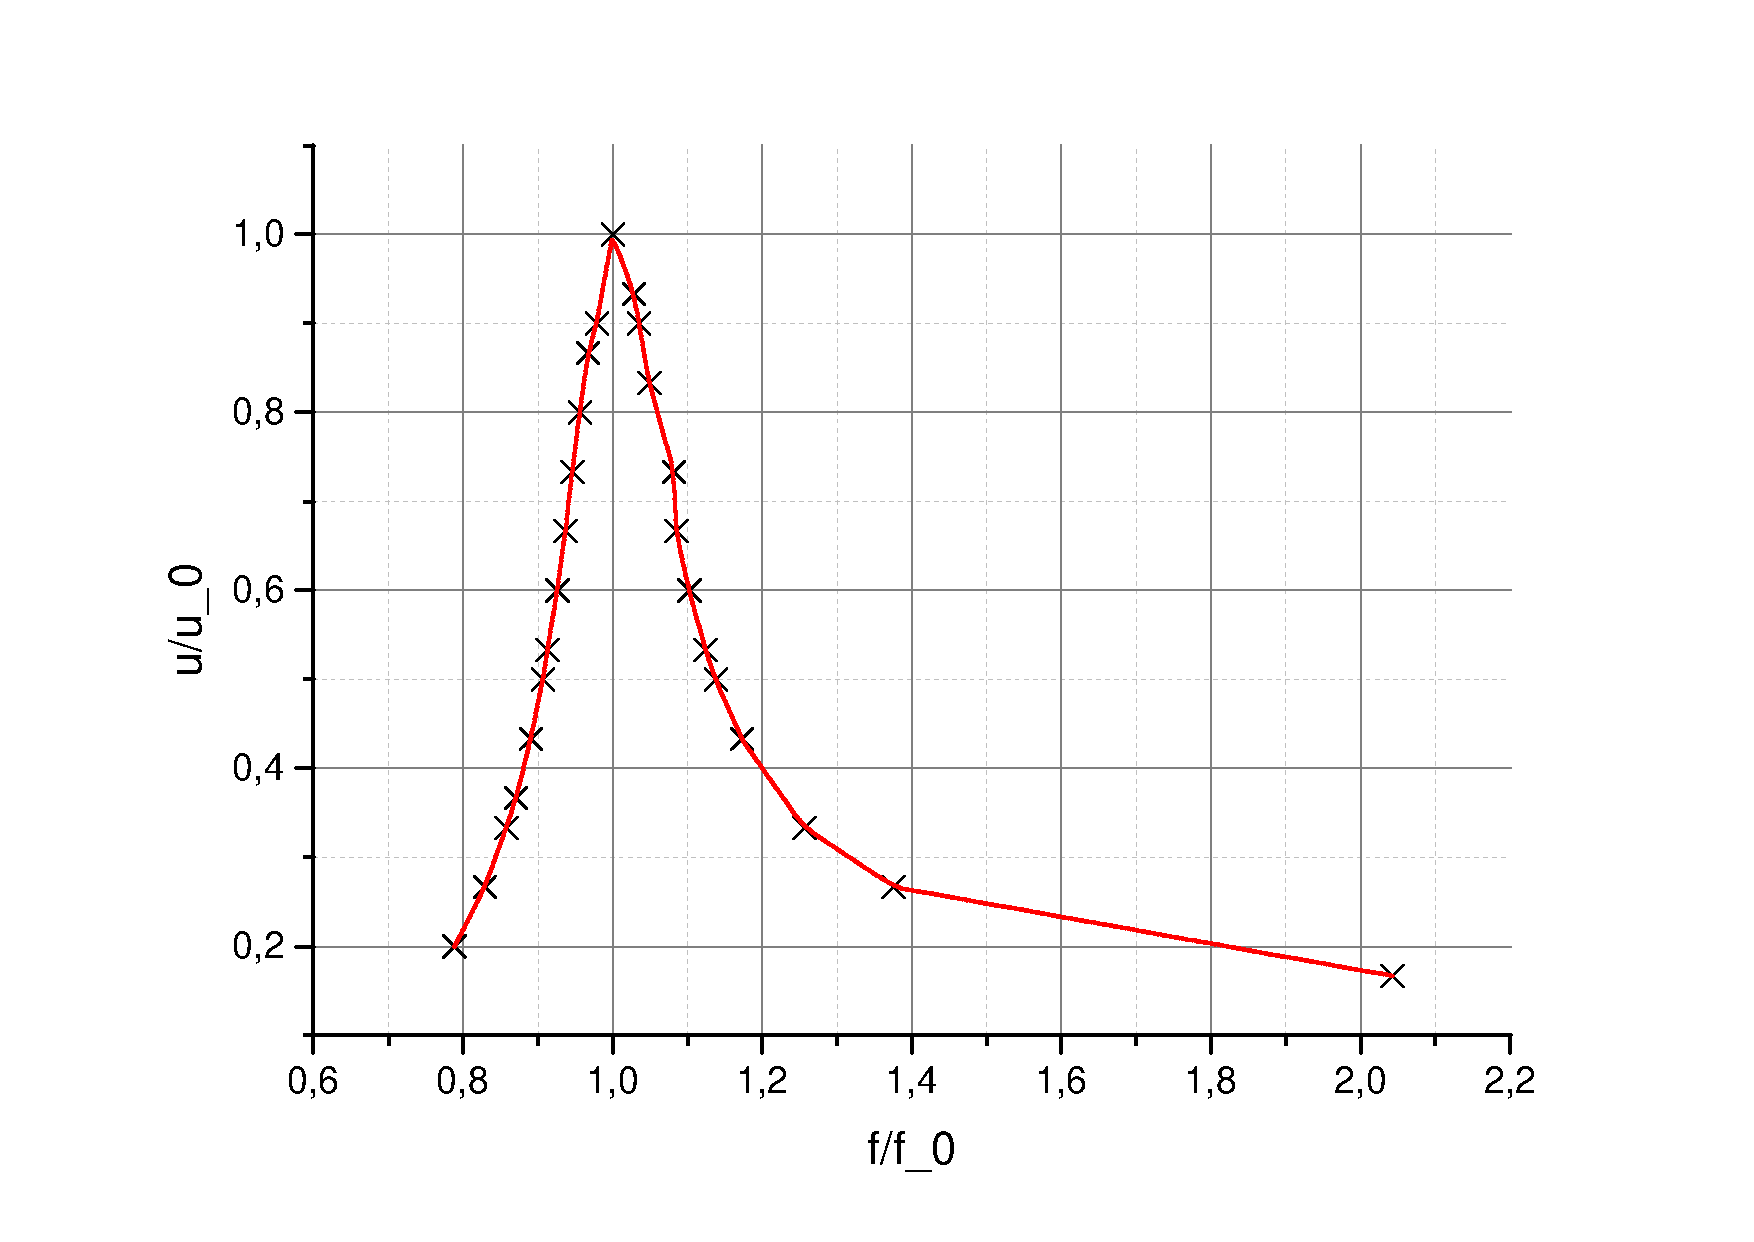
\includegraphics[width = 0.7\linewidth]{graph2}
		
		
		\subsection{Процессы установления и затухания колебаний}
		Сделаем измерения:
		
	\begin{table}[h]
		\begin{tabular}{| l | l | l | l || l | l |}
			\hline
			R = 0 Ом  &      &      &      & R = 100 Ом &      \\ \hline
			n         & 5    & 6    & 8    & 3          & 2    \\ \hline
			$V_n$     & 0.2  & 0.08 & 0.4  & 0.03       & 0.08 \\ \hline
			$V_{k+n}$ & 0.3  & 0.27 & 0.28 & 0.1        & 0.11 \\ \hline
			$V_0$     & 0.31 & 0.31 & 0.31 & 0.12       & 0.12 \\ \hline
			$V_{m}$   & 0.15 & 0.1  & 0.2  & 0.06       & 0.12 \\ \hline
			$V_{k+m}$ & 0.1  & 0.06 & 0.1  & 0.02       & 0.05 \\ \hline
		\end{tabular}
	\end{table}
	
	Теоретическая добротность:
	
	Q = $\frac{1}{R}\sqrt{\frac{L}{C}} \implies Q_0 = 45.59, \quad Q_{100} = 8.22$
	
	Добротность по графику:
	$Q_0 = 34.58, \quad Q_{100} = 7.12$
	
	Добротность по огибающим:
	$Q_0 = 38.74, \quad Q_{100} = 7.82$
	
	\section{Вывод}
		В колебательном контуре, подключенном к источнику синусоидального напряжения, через некоторое время собственные колебания затухают. Наибольшие по амплитуде вынужденные колебания наблюдаются при совпадении собственной и вынуждающей частоты.
		
\end{document}


